\chapter{Background and Related Work}
\label{sec:background}

In this section, we review some of the background critical to this proposal.
We begin with a discussion of Recognizing Textual Entailment and the core
motivation of our thesis.  We then overview Distributional Semantics, outlining
its purpose and one common implementation of VSMs. Finally, we discuss the
Lexical Entailment (LexEnt) and Lexical Substitution (LexSub) tasks, which we
view as two useful proxies for the kinds of lexical semantics necessary in
RTE. We do not argue that these tasks are completely sufficient, but one goal
of our thesis to show that developments in these tasks improves practical RTE.

\section{Recognizing Textual Entailment}
\label{sec:textent}

In the Introduction, we introduced the Recognizing Textual Entailment (RTE)
task as a long standing, challenging semantic problem in the field of
Natural Language Processing.  One of the first benchmark papers describes RTE
as ``recognizing, given two text fragments, whether the meaning of one text can
be inferred (entailed) from the other'' \cite{dagan:2006:mlc}. Since this
original definition, many other datasets
\cite{giampiccolo:2007:pascal,bentivogli:2009:tac,marelli:2014:semeval} and
countless approaches have been described (c.f. \newcite{dagan:2013:synthesis}
for a thorough survey). Although RTE is not usually considered an
end-user application by itself, successful RTE systems could influence many
downstream tasks like Information Extraction or Question Answering and become
useful in information-heavy industries like defense, journalism, and science.

RTE is a very difficult task, at least partially due to its generality.
Entailment reasoning may require: broad common sense knowledge or highly
specialized domain knowledge; sophisticated logical inferences
about quantifiers and implication; or more graded, fuzzier reasoning about
related words. In our own work, we focus predominantly on some of the issues
of {\em lexical semantics} necessary for reasoning in RTE systems. These
include issues like lexical relationship detection, where one must classify
{\em how} two words are (or are not) related, and lexical paraphrasing, where
one must suggest alternative words which have the same meaning.

Presently, RTE systems often employ a wide collection of lexical resources in
order to capture some of these issues in lexical semantics
\cite{maccartney:2008:coling,bjerva:2014:semeval,beltagy:2016:cl}. These
rich lexical resources, including WordNet \cite{miller:1995:acm} and PPDB
\cite{ganitkevitch:2013:naacl}, provide an excellent
source of common sense knowledge and word relationships which can be used as a
background knowledge-base during logical reasoning. In our work, we consider
whether it is possible to distill information about lexical relationships
automatically.  We turn now to Distributional Semantics and Vector Space
Models, which provide an automatic induction of word meaning using only large,
unannotated corpora.

\section{Distributional Semantics}
\label{sec:dist}

Distributional Semantics is a powerful tool for automatically inducing semantic
representations for lexical items \cite{turney:2010:jair,erk:2012:llc}.  The
core notion is that of the {\em Distributional Hypothesis}, that if two words
appear in similar {\em contexts}, they can be assumed to have similar meaning.
This idea has a long history in the linguistic and philosophical literature that
can be traced back over 60 years
\cite{wittgenstein:1953:pi,harris:1954:word,firth:1957:la}. In its modern form,
Distributional Semantics involves finding {\em vector space representations} of
words which are constructed by counting or modeling the contexts in which a
particular word appears. According to the Distributional Hypothesis, words
with similar {\em vectors} can be assumed to have similar {\em meanings}
\cite{turney:2010:jair}. For this reason, they are often referred to as
Vector Space Models (VSMs) of language. Variations on this idea have also
become immensely popular in the neural networks community, with algorithms
like Skip-gram Negative Sampling (SGNS) \cite{mikolov:2013:iclr} and GloVe
\cite{pennington:2014:emnlp}, and have often replaced traditional count-based
VSMs in the NLP community \cite{baroni:2014:acl}.

\begin{figure}
\centering
\begin{minipage}{7cm}
\begin{scriptsize}
\begin{alltt}
         the furry {dog} is friendly to
and manipulate the {dog} 's lips and
       as a clever {dog} ; two to
a reputation among {dog} trainers of having
    also among the {dog} breeds most likely
 the very earliest {dog} shows and kennel
        as a guard {dog} and to hunt
   the mechanic 's {dog} began to howl
\end{alltt}
\end{scriptsize}
\end{minipage}\qquad
\begin{minipage}{3cm}
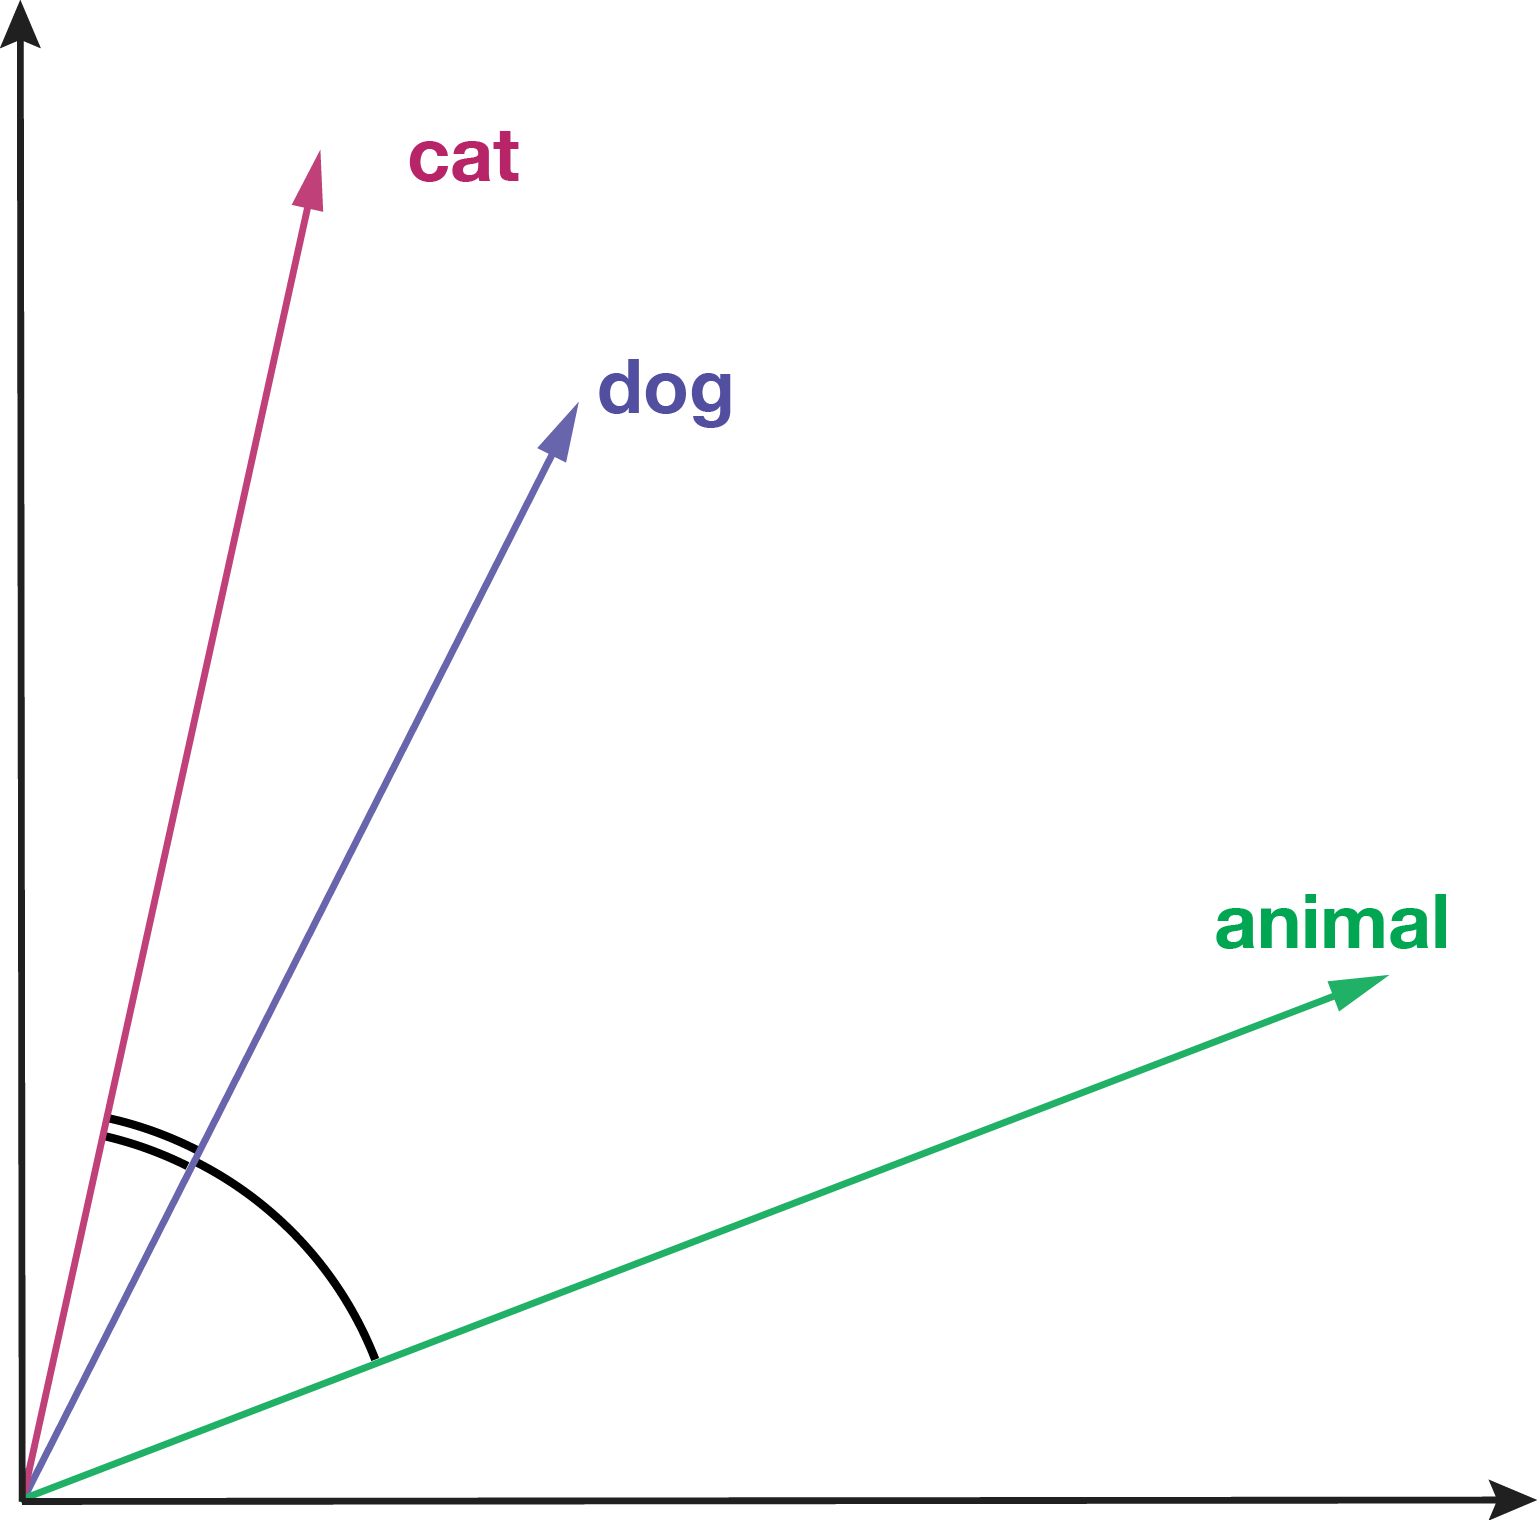
\includegraphics[width=3cm]{figures/vsm}
\end{minipage}
\caption{(a) Example contexts of the word {\em dog}, and (b) a cartoon drawing
of word vectors.}
\label{fig:vsm}
\end{figure}

In its simplest form, vectors are induced by defining a vector space where
each dimension in the space corresponds to a particular context word. A large,
unannotated corpus of text is then processed, finding instances of a target word,
like {\em dog}, and incrementing a count for each of the target's {\em
co-occurrences}, or words appearing around the target word
{\em dog}, as in Figure~\ref{fig:vsm}. With a large enough corpus, coherent
statistical patterns begin to form. For example, the word {\em furry} is likely
to be used to describe both {\em cat} and {\em dog}, which is then reflected in
the vector counts \cite{lund:1996:brmic}. After constructing vector
representations for the words {\em cat} and {\em dog}, we can then compare
these vectors using various geometric distance metrics, most prominently {\em
cosine similarity}:
\begin{equation}
  \text{cosine}(u, v) = \frac{\sum_i u_iv_i}{\sqrt{\sum_i u_i^2 \sum_i v_i^2}}
  \label{eq:cos}
\end{equation}
Here, $i$ iterates over all the different context dimensions, like {\em furry}
or {\em kennel}, and cosine similarity is defined over the range $[-1, 1]$.
Words with similar vectors will have a smaller angle between them, and therefore
a higher cosine similarity (i.e. close to 1).

\paragraph{Count Transformations}
In practice, usually the distributional vectors are more sophisticated in their
construction than raw co-occurrence counts.  Typically, words and contexts
below a certain threshold are omitted from the co-occurrence matrix, because
extremely rare words have few counts and therefore impoverished representations
\cite{turney:2010:jair}. The co-occurrence matrix is also usually transformed
using some nonlinearity; one common choice is Positive Pointwise Mutual
Information (PPMI) \cite{bullinaria:2007:brm}, where the raw co-occurrence count
between a word $w$ and context $c$ is transformed,
\begin{equation*}
  \text{PPMI}(w, c) = \max\left(0, \log\frac{P(w, c)}{P(w)P(c)}\right)
\end{equation*}
Pointwise Mutual Information (PMI) measures roughly how many times more likely two
items co-occur more often than chance, while Positive PMI
additionally ignores co-occurrences that occur less often than chance.  Other
transformations, like conditional probability
\cite{hofman:1999:sigir,blei:2003:jmlr} and Softplus
\cite{pennington:2014:emnlp}, are also sometimes seen in the literature, and
emphasize different aspects of lexical similarity.

\paragraph{Syntactic Contexts}
Defining contexts is another important aspect of Distributional Semantics.
In the example of Figure~\ref{fig:vsm}, we showed that context can be defined
as three words to the left and right of the target word, but there are
alternatives. For example, using very large windows of co-occurrence (or even
entire documents) results in emphasizing more {\em topical} similarity, e.g. doctor
and hospital, while smaller windows emphasize more {\em functional} similarity, e.g.
doctor and surgeon \cite{pado:2007:cl,erk:2008:emnlp,levy:2014:acl}.

Context can be also defined as {\em syntactic neighbors} extracted from a
dependency parse. For example, in Figure~\ref{fig:syn}, the
contexts for the word {\em chased} would be {\em nsubj+dog} and {\em
dobj+tail}. Distributional Spaces defined in this manner tend to emphasize the
{\em selectional preferences} of words, or the tendency of words to have
particular arguments in their syntactic relations.
\cite{pado:2007:cl,erk:2008:emnlp,baroni:2010:cl,levy:2014:acl}. For example,
the subject of {\em barks} is likely to be {\em dog}, while the subject of
{\em purrs} is likely to be {\em cat}.

\begin{figure}
  \centering
  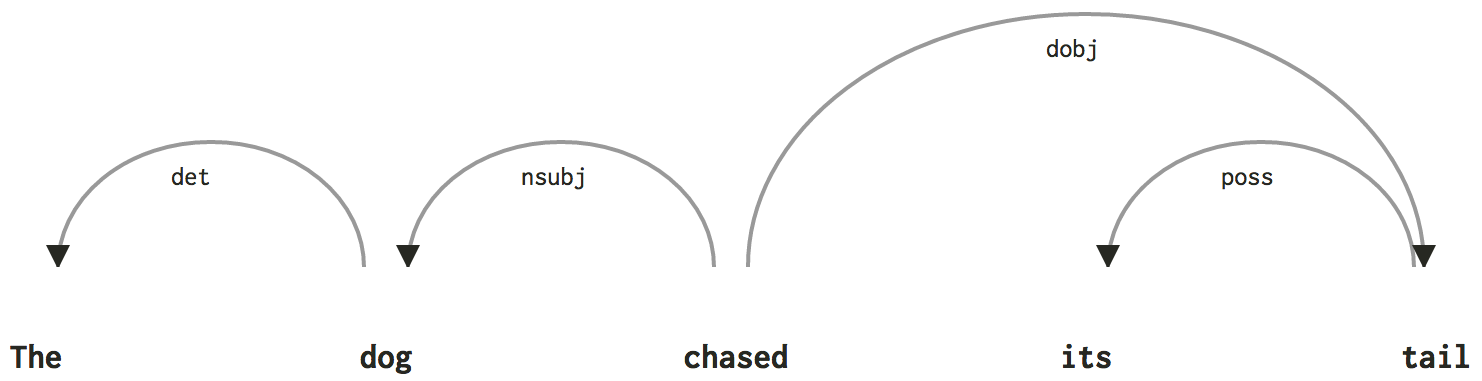
\includegraphics[width=0.75\textwidth]{figures/syn}
\caption{Example of a dependency parse for ``The dog chased its tail.'' In
a syntactic distributional space, contexts are defined as adjacent nodes
with their labeled edges.}
\label{fig:syn}
\end{figure}

\paragraph{Dimensionality Reduction}
Dimensionality Reduction is another important aspect of Distributional Semantics.
As described earlier, distributional vector
spaces are very high-dimensional: bag-of-words spaces have many thousands of
dimensions \cite{turney:2010:jair,mikolov:2013:iclr,pennington:2014:emnlp},
while syntactic spaces usually have a millions \cite{baroni:2010:cl}.
Efficiently dealing with these large, extremely sparse vectors can be
troublesome, so we often opt to use some form of {\em dimensionality
reduction}, like Singular Value Decomposition (SVD)
\cite{deerwester:1990:jsis,landauer:1997:pr} or Nonnegative Matrix
Factorization (NNMF) \cite{lee:2000:nips}. In dimensionality reduction, the
co-occurrence matrix $M$ is typically assumed to be factorizable into two
lower-rank matrices,
\begin{equation}
  M = VC^{\top}
  \label{eqn:svd}
\end{equation}
where $V$ is some lower dimension representation of word vectors, and $C$ is
the corresponding lower dimension representation of the context items. These
projections of words and contexts into the same latent space traces back to the
earliest days of distributional semantics \cite{deerwester:1990:jsis}, and is
critical to many of the contributions of our completed work.  Interestingly,
the most popular algorithms for computing word embeddings, like Skip-Gram
Negative Sampling (SGNS) \cite{mikolov:2013:iclr} and GloVe
\cite{pennington:2014:emnlp} can be viewed as form of dimensionality reduction
\cite{levy:2014:nips,levy:2015:tacl}.

\section{Lexical Entailment and Relationship Detection}

To paraphrase \newcite{shnarch:2008:thesis}, Lexical Entailment may be broadly
defined as any number of semantic relations between two lexical items where the
meaning of one is implied by the meaning of another.
This includes many classical lexical relations, like hypernymy
({\em a girl} is a {\em child}; {\em a dog} is an {\em animal}), and meronomy
({\em a girl} has {\em eyes}; {\em a dog} has a {\em tail}), but it can also include a
wide variety other inferences which are difficult to categorize,
like {\em to snore} implies {\em to sleep}.

As shown in our example
sentence in the Introduction, understanding and predicting these lexical relationships
is critical to performing certain inferences in RTE: without basic lexical
relationships, even the easiest textual entailments would be out of
reach. There has been a great deal of research around predicting lexical
relationships automatically from text. We cannot possibly enumerate all the
work on this problem, but we aim to cover some influential approaches and to
emphasize attempts related to distributional semantics

One important, early development in this task was Hearst patterns
\cite{hearst:1992:coling}, which are specific textual patterns highly
indicative of particular relationships. Common Hearst patterns include
exemplar phrases like ``X such as Y,'' ``X including Y,'' which are both highly
indicative of hypernymy. Possessive phrases, like ``X's Y'', can be indicative
of meronomy. Later,
\newcite{snow:2004:nips} extended this Hearst pattern approach
to use syntactic patterns. By using syntactic parses, some longer distance patterns
are more easily captured, like ``X such as Y and Z,'' which implies ``X such as Z.''

More recently, groups have begun researching how lexical relationships may be
mined automatically using VSMs. Since Distributional
Semantics provides a way of estimating word meaning automatically from only
large, unannotated corpora, they may also be able to identify
word relationships \cite{baroni:2011:gems,baroni:2012:eacl}. Ideally, this
could be used to augment existing lexical resources like WordNet, bootstrap
a WordNet-like resource in new languages, and help downstream tasks like RTE
and QA.

Early work in predicting lexical entailments using distributional spaces was
focused mostly on attempts to find unsupervised similarity measures to identify
hypernymy from word vectors
\cite{weeds:2004:coling,clarke:2009:gems,kotlerman:2010:nle,lenci:2012:starsem,santus:2013:thesis}.
The reasoning was that with the right corpus, the right
distributional space, and the right similarity measure, hypernym pairs
(or at least candidate pairs) could be readily identified using only word
vectors. This view was developed in part by evidence that the ubiquitous
cosine similarity tends to highlight co-hyponym pairs more than other relations
\cite{weeds:2004:coling,baroni:2011:gems}.  One lasting hypothesis about
hypernymy detection has been the Distributional Inclusion Hypothesis (DIH)
\cite{zhitomirsky-geffet:2005:acl}, which states that the contexts in which a
hypernym appears should be a superset of all its hyponyms. A considerable
amount of work assumed the DIH to be at least partially true, and many of the
proposed measures were based on the Distributional Inclusion Hypothesis in one
form or another \cite{clarke:2009:gems}, or a hybrid of DIH and cosine
similarity \cite{kotlerman:2010:nle,lenci:2012:starsem}.

As it became obvious that unsupervised measures did not work as
well as hoped, the community began working on entailment detection as a
supervised task. \newcite{baroni:2012:eacl} proposed, as a preliminary baseline
of a novel dataset, training a simple baseline classifier to predict whether
word pairs were either hypernyms or non-hypernyms. Although they reported strong performance,
others later realized their model struggled with issues of {\em lexical
memorization}, or a special kind of overfitting
\cite{roller:2014:coling,weeds:2014:coling,levy:2015:naacl}. As such, more
recent works have emphasized their performance when {\em individual words are
held out entirely}, so that the same word can never appear in both training and
testing sets
\cite{roller:2014:coling,kruszewski:2015:tacl,levy:2015:naacl,shwartz:2016:acl,roller:2016:naacl}.
We discuss more about this issue of Lexical Memorization in
Section~\ref{sec:lexmem}.

\section{Lexical Substitution}
\label{sec:lexsub}

In our discussion of lexical relationships, we assumed that words are
mononymous, or that they have only one meaning. However, words like ``bright''
have multiple meanings, which change depending on context, as in ``bright
girl'' and ``bright coat.'' This is called {\em polysemy}, and is a major issue
in Natural Language Understanding, since it adds another layer of ambiguity.

One approach to dealing with polysemy is to model how word
meaning {\em shifts} in a given context; that is, we can explicitly model what
happens to a word based on its use in a sentential context. Since 2007, one
popular way to measure this has been the Lexical Substitution task.  In the
Lexical Substitution task, we are provided with a sentential context,
and must suggest {\em substitutes} which can replace the given target word,
while preserving the meaning of the entire sentence
\cite{mccarthy:2007:semeval,biemann:2012:lrec,kremer:2014:eacl}.

At first glance, the Lexical Substitution task has a less obvious connection to
Textual Entailment than the Lexical Entailment task does. However, we argue
it is also an important proxy to improvements on Textual Entailment, and that
Lexical Substitution may act as a kind of lexical entailment {\em
in context}: if a substitute can replace the target and preserve the meaning of
the sentence, then it follows that the target {\em entails} the substitute.
Although this includes basic synonymy (like ``bright'' and ``clever''), it
also covers much more interesting specialized cases. For example, with the
context
\begin{quote}
  ``Tara stood stock-still, waiting for the first tiny gleam from the
  scout craft to appear in the darkness of the {\bf wormhole},''
\end{quote}
human annotators considered {\em portal} and {\em rift} to be excellent
substitutes. These substitutes take into account the Science Fiction context of the
sentence, indicating the task is more complicated than simple synonymy. Indeed,
\newcite{kremer:2014:eacl} found that only 9\% of substitutes in their dataset were
direct synonyms in WordNet.  For this reason, we believe that Textual
Entailment can benefit more from modeling Lexical Substitution as a complete
task, rather treating the phenomenon as explicit lexical relations.

Distributional Semantics offers a tempting solution to this problem of Lexical
Substitution, given its ability to measure the {\em graded} levels of similarity
between words \cite{erk:2008:emnlp}. Interestingly, although there have been
both supervised \cite{biemann:2012:lrec,szarvas:2013:naacl} and unsupervised
attempts
\cite{erk:2008:emnlp,dinu:2010:emnlp,thater:2010:acl,vandecruys:2011:emnlp,kremer:2014:eacl,melamud:2015:naacl,melamud:2015:vsm,kawakami:2016:iclr,roller:2016:naacl}
using distributional semantics, presently unsupervised measures hold
a lead \cite{melamud:2015:naacl,melamud:2016:conll}.


